\documentclass{article}
\usepackage{amsmath, amssymb, graphicx}

\begin{document}

The other vision-based model we propose is based on the Segment Anything Model (SAM). SAM is a foundation model for image and videos segmentation. Developed by Meta's FAIR (Fundamental AI Research) lab, SAM represents a significant advancement in computer vision, designed to serve as a versatile framework for various segmentation tasks. His architecture can be summarized in three parts: a Vision Transformer image encoder, a prompt encoder, and a modified mask Transformer decoder block (see Figure \ref{label}).

\begin{figure}[h!]
    \centering
    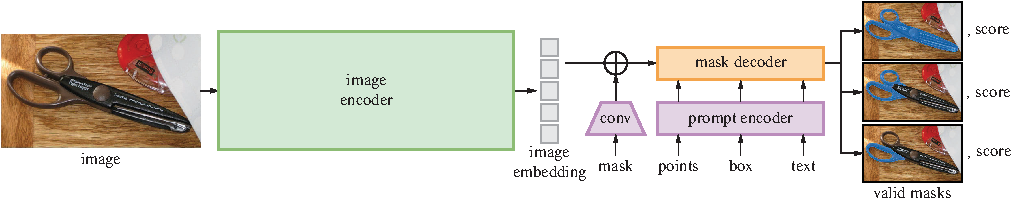
\includegraphics[width=1\linewidth]{figures\model_diagram.pdf}
    \caption{Segment Anything Model (SAM) overview}
    \label{label}
\end{figure}

Now, to address the task, we first produce a high-quality image using the GeoJSON-to-Image pipeline presented earlier. Then, we use SAM to infer masks on the image as segmentation of all the rooms. Finally, the contours of the masks are extracted, and after rescaling the contour coordinates, we generate the corresponding GeoJSON file. This process essentially reverses the GeoJSON-to-Image pipeline, completing the cycle from GeoJSON to image and back to GeoJSON. In Table \ref{tab:model_checkpoint}, we find the SAM model checkpoint used.

\begin{table}[h]
    \centering
    \begin{tabular}{|l|l|}
        \hline
        \textbf{Checkpoint} & \texttt{sam\_vit\_h\_4b8939.pth} \\ \hline
        \textbf{Backbone Size} & Huge (ViT-H) \\ \hline
        \textbf{Model Parameters} & 636 million \\ \hline
        \textbf{File Size} & 2.4 GB \\ \hline
        \textbf{GPU Memory Requirement} & At least 8 GB \\ \hline
        \textbf{Use Case} & Tasks requiring high-quality segmentations \\ \hline
    \end{tabular}
    \caption{Model Checkpoint Information}
    \label{tab:model_checkpoint}
\end{table}


\end{document}